\documentclass[14pt, a4paper]{report}
\usepackage{mathtext}
\usepackage[T2A]{fontenc}
\usepackage[utf8]{inputenc}
\usepackage[russian]{babel}
\usepackage{multirow}
\usepackage{slashbox}
\usepackage{makecell}
\usepackage{graphicx}
\usepackage{physics}
\usepackage{amstext}
\usepackage{caption}
\usepackage{subcaption}
\usepackage{cmap}
\usepackage{float}

\renewcommand{\thesection}{\arabic{section}.}
\renewcommand{\thesubsection}{\arabic{section}.\arabic{subsection}.}

\title{\textbf{Отчет о выполнении лабораторной работы 2.2/2.3 "Изучение спектров атома водорода и молекулы йода"}}
\author{Калашников Михаил, Б03-202}
\date{}

\begin{document}
\maketitle

\textbf{Цель работы:}
Исследовать спектральные закономерности в оптическом спектре водорода и спектр поглощения паров йода в видимой области.
\newline


\textbf{В работе используются:}
\begin{itemize}
\item стеклянно-призменный монохроматор-спектрометр УМ-2;
\item собирающая линза;
\item неоновая лампа;
\item ртутная лампа ДРШ;    
\item водородная лампа;
\item лампа накаливания К12;
\item кювета с йодом;
\end{itemize}

\section{Теоретические сведения}

\subsection{Спектр водорода}

Атом водорода является простейшей атомной системой. Поэтому спектр водорода является предметом тщательного экспериментального и теоретического исследования. Энергии квантов спектральных линий атома водорода описываются формулой:

\[E=R(\frac{1}{n^2}-\frac{1}{m^2}),\]

где $R$ -- константа, называемая постоянной Ридберга, а $n$ и $m$ -- целые числа.

\begin{figure}[H]
\centering
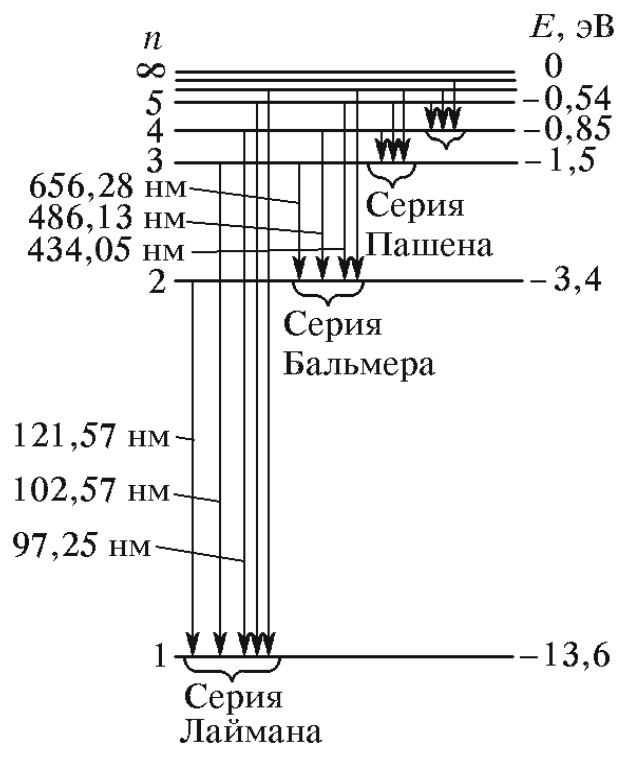
\includegraphics[scale=0.3]{../images/523-5}
\caption{Уровни энергии атома водорода и образование спектральных серий}
\end{figure}

В данной работе будет изучена серия Бальмера, линии которой лежат в видимой области спектра. Для первых четырех линий серии Бальмера величины  $n$ и $m$ принимают значения 2 и 3, 4, 5, 6 соответственно. Эти линии обозначаются символами $H_\alpha$, $H_\beta$, $H_\gamma$, $H_\delta$.

\subsection{Спектр йода}

Молекулы обладают более богатым спектром возбужденных состояний, чем изолированные атомы. В молекулах могут возбужаться дополнительные степени свободы: колебания составляющих их атомов относительно друг друга и вращения молекул относительно различных осей.

Можно показать, что характерная энергия вращательных движения в $10^6$ раз меньше энергии электронных переходов, и поэтому наблюдение вращательных переходов оптическими спектрометрами невозможно. В видимой области наблюдается наложение колебательного спектра на электронный. Каждой линии электронного перехода соответствует ряд колебательных линий, образующих полосу.

\begin{figure}[H]
\centering
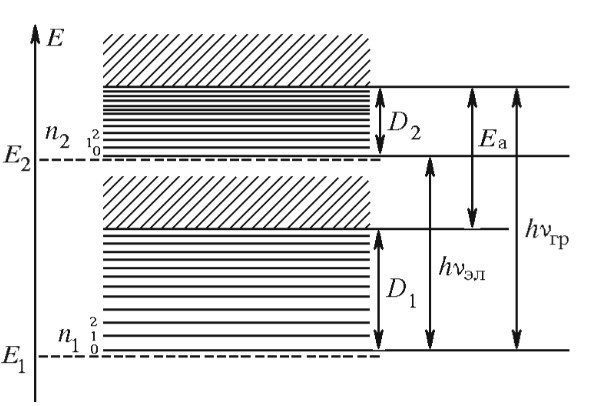
\includegraphics[scale=0.5]{../images/523-6}
\caption{Электронные и электронно-колебательные энергетические уровни двухатомной молекулы}
\end{figure}

Штриховыми линиями показаны электронные уровни, а сплошными -- колебательные подуровни этих состояний. С ростом квантовых чисел  $n_1$ и $n_2$ колебательные уровни сближаются и переходят в непрерывный спектр, области которого заштрихованы на рисунке. Так же растет и амплитуда колебаний, при достижении некоторой максимальной амплитуды проиходит диссоциация молекулы.

\section{Экспериментальная установка}

В работе используется стеклянно-призменный монохроматор-спектрометр УМ-2, предназначенный для спектральных исследований в диапазоне от 0.38 до 1.00 мкм. Рассмотрим основные элекменты монохроматора:

\begin{enumerate}

\begin{figure}[H]
\centering
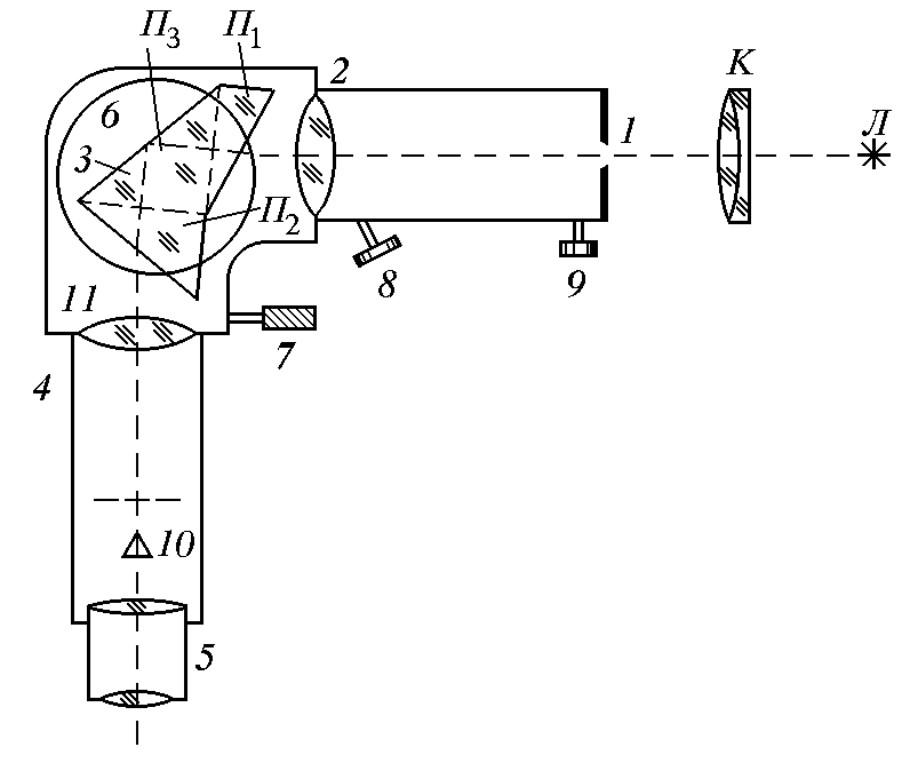
\includegraphics[scale=0.3]{../images/523-3}
\caption{Схема экспериментальной установки}
\end{figure}

\item Входная щель 1, снабженная микрометрическим винтом 9, позволяющим реулировать ширину открытия щели.

\item Коллиматорный объективный 2, снабженный микрометрическим винтом 8, позволяющим смещать объектив при фокусировке спектральных линий различных цветов.

\item Спектральная призма 3, установленная на поворотном столике 6.

\item Поворотный столик 6, вращающийся при помощи микрометрического винта 7 с отсчетным барабаном.

\item Зрительная труба из объектива 4 и окуляра 5. В фокальной плоскости объектива расположено острие указателя.

\item Корпус 11.

\item Оптическая скамья, на которой могут перемещаться рейтеры с линзой-конденсером, различными источниками света и кюветой с йодом.

\end{enumerate}

\section{Проведение эксперимента}

\subsection{Подготовка установки к работе}

\begin{enumerate}

\setcounter{enumi}{0}

\item Ознакомимся с устройством и принципом работы спектрометра

\item Включим неоновую лампу. Отцентрируем оптическую систему

\item Расположим конденсор так, чтобы получить резкое изображение источника в центре колпачка, прикрывающего входную щель. Закрепим рейтеры.

\item Вращая глазную линзу окуляра, настроимся на рекое изображение кончика указателя.

\item Вращая барабан, подведем указатель к одной из ярких линий неона. Перемещая коллиматор, получим четкое изображение линии.

\item Установим ширину входной щели так, чтобы получить наиболее резкое изображение спектральных линий.

\end{enumerate}

\subsection{Градуировка спектрометра}

\begin{enumerate}

\setcounter{enumi}{0}

\item Откалибруем спектрометр по спектру неона при помощи таблицы с расположение спектральных линий.

\item Проделаем то же самое по спектру ртути с помощью ртутной лампы.

\end{enumerate}

\subsection{Спектр водорода}

\begin{enumerate}

\setcounter{enumi}{0}

\item Установим на скамью водородную лампу и включим ее в сеть.

\item Измерим положение линий $H_\alpha$, $H_\beta$, $H_\gamma$, $H_\delta$.

\end{enumerate}

\subsection{Спектр йода}

\begin{enumerate}

\setcounter{enumi}{0}

\item Установим на лампу накаливания К12 и кювету с йодом. Отцентрируем полученное изображение на колпачке входной щели.

\item Настроим установку так, чтобы на ярком фоне непрерывного спектра наблюдались темные полосы поглощения.

\item Определим деления барабана монохроматора, соответствующие линиям: $\nu_{1,0}$ -- самой длинноволновой видимой линии поглощения, $\nu_{1,5}$ -- шестой по счету длинноволновой видимой линии поглощения и $\nu_{гр}$ -- границе схождения спектра.

\end{enumerate}

\section{Обработка результатов}

\begin{enumerate}

\setcounter{enumi}{0}

\item Построим калибровочную кривую. Для этого отложим на графике точки, полученные при измерении спектров неона и ртути. Через точки проведем функцию, заданную дисперсионной формулой Гартмана:

\[\lambda=\lambda_0+C/(d-d_0),\]

где $\lambda_0$, $C$ и $d_0$ -- три постоянные, подбираемые с помощью МНК.

\begin{figure}[H]
\centering
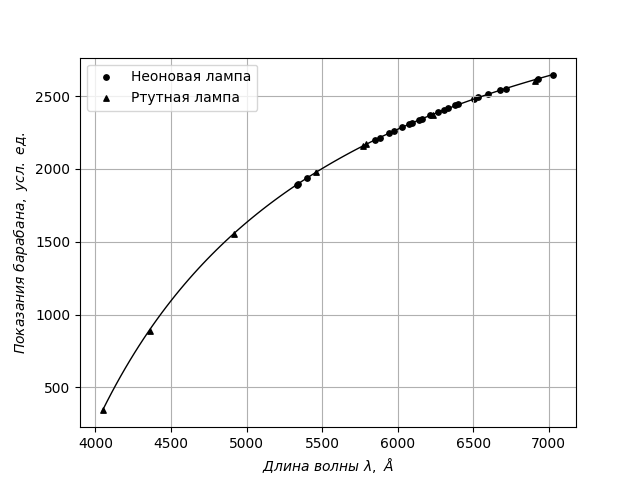
\includegraphics[scale=0.6]{../images/523-1}
\caption{Калибровочная кривая монохроматора-спектрометра}
\end{figure}

\item По калибровочной кривой определим длины волн линий $H_\alpha$, $H_\beta$, $H_\gamma$, $H_\delta$.
Погрешность найдем по формуле погрешности косвенных измерений:
\[\sigma_\lambda=\sqrt{\sigma_{\lambda_0}^2+\left(\frac{\lambda-\lambda_0}{C}\right)^2\left(\sigma_C^2+(\lambda-\lambda_0)^2\sigma_{d_0}^2\right)}\]

\[\lambda_{H_\alpha}=(653\pm4)\ нм,\quad\lambda_{H_\beta}=(486\pm2)\ нм,\]
\[\lambda_{H_\gamma}=(433.7\pm1.7)\ нм,\quad\lambda_{H_\delta}=(409.8\pm1.5)\ нм.\]

\item Убедимся в том, что отношения длин волн линий соответствуют формуле сериальной закономерности ($m\ge3$):

\[\frac{\lambda_{H_m}}{\lambda_{H_{m+1}}}=\frac{\frac{1}{2^2}-\frac{1}{(m+1)^2}}{\frac{1}{2^2}-\frac{1}{m^2}}=\frac{(m-1)m^2(m+3)}{(m-2)(m+1)^2(m+2)}\]

\[\left(\frac{\lambda_{H_\alpha}}{\lambda_{H_\beta}}\right)_{th}=1.35,\quad\frac{\lambda_{H_\alpha}}{\lambda_{H_\beta}}=1.343\pm0.014,\]
\[\left(\frac{\lambda_{H_\beta}}{\lambda_{H_\gamma}}\right)_{th}=1.12,\quad\frac{\lambda_{H_\beta}}{\lambda_{H_\gamma}}=1.120\pm0.009,\]
\[\left(\frac{\lambda_{H_\gamma}}{\lambda_{H_\delta}}\right)_{th}\approx1.058,\quad\frac{\lambda_{H_\gamma}}{\lambda_{H_\delta}}=1.059\pm0.008.\]

\item Отложим на графике точки зависимости энергии перехода ($E=h\frac{c}{\lambda}$) от параметра $1/2^2-1/m^2$. По наклону прямой, проведенной через точки определим постоянную Ридберга. Получим:

\[R=(13.529\pm0.016)\ эВ.\]

\begin{figure}[H]
\centering
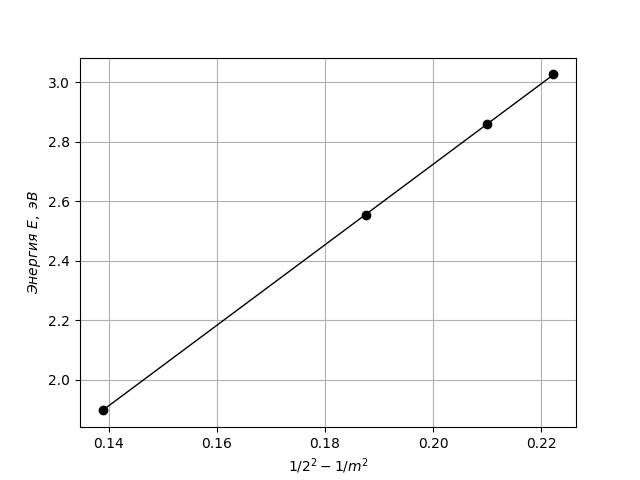
\includegraphics[scale=0.6]{../images/523-2}
\caption{Зависимость энергии перехода от параметра}
\end{figure}

\item Воспользуемся калибровочной кривой для определения длин волн линий $\lambda_{1,0}$. $\lambda_{1,5}$, $\lambda_{гр}$:

\[\lambda_{1,0}=(607\pm3)\ нм,\quad \lambda_{1,5}=(584\pm3)\ нм,\quad \lambda_{гр}=(500\pm2)\ нм.\]

\item Вычислим энергию колебательного кванта возбужденного состояния молекулы йода:

\[h\nu_2=\frac{h\nu_{1,5}-h\nu_{1,0}}{5}=(0.015\pm0.004)\ эВ.\]

Также вычислим энергию $h\nu_{гр}=h\frac{c}{\lambda_{гр}}=(2.481\pm0.011)\ эВ$.

\item Зная, что энергия колебательнго кванта основного состояния $h\nu_1=0.027\ эВ$, а энергия возбуждения атома $E_A=0.94\ эВ$, вычислим:

\begin{enumerate}

\item энергию электронного перехода:

\[h\nu_{эл}=E_2-E_1=h\nu_{1,0}+\frac{3}{2}h\nu_{1}-\frac{1}{2}h\nu_{2}=(2.077\pm0.012)\ эВ,\]

\item энергию диссоциации молекулы в основном состоянии:

\[D_1=h\nu_{гр}-E_A=(1.541\pm0.011)\ эВ,\]

\item энергию диссоциации молекулы в возбужденном состоянии:

\[D_2=h\nu_{гр}-h\nu_{эл}=(0.40\pm0.02)\ эВ.\]

\end{enumerate}

\begin{figure}[H]
\centering
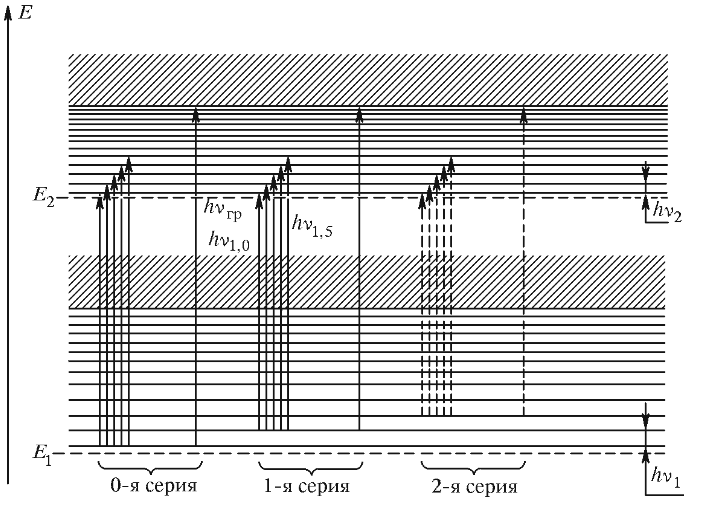
\includegraphics[scale=0.6]{../images/523-4}
\caption{К вычислению энергий перехода и диссоциации}
\end{figure}

\end{enumerate}

\section{Выводы}

Сравним полученные результаты с табличными. В лабораторном практикуме приведены следующие значения $D_1$ и $D_2$:
\[D_1=1.5425\ эВ,\quad D_2=0.69\ эВ\]
Можно сделать вывод о том, что в результате проделанной работы энергия диссоциации молекулы в основном состоянии найдена с более высокой точностью, по сравнению с энергией диссоциации в возбуджденном состоянии.

\end{document}